\documentclass[journal]{IEEEtran}
\usepackage{blindtext}
\usepackage{graphicx}
\usepackage{todonotes}
\usepackage{cite}
\usepackage[cmex10]{amsmath}
\usetikzlibrary{calc,positioning}

\newcommand{\clash}{C$\lambda$aSH}


% *** ALIGNMENT PACKAGES ***
%
%\usepackage{array}
% Frank Mittelbach's and David Carlisle's array.sty patches and improves
% the standard LaTeX2e array and tabular environments to provide better
% appearance and additional user controls. As the default LaTeX2e table
% generation code is lacking to the point of almost being broken with
% respect to the quality of the end results, all users are strongly
% advised to use an enhanced (at the very least that provided by array.sty)
% set of table tools. array.sty is already installed on most systems. The
% latest version and documentation can be obtained at:
% http://www.ctan.org/tex-archive/macros/latex/required/tools/


%\usepackage{mdwmath}
%\usepackage{mdwtab}
% Also highly recommended is Mark Wooding's extremely powerful MDW tools,
% especially mdwmath.sty and mdwtab.sty which are used to format equations
% and tables, respectively. The MDWtools set is already installed on most
% LaTeX systems. The lastest version and documentation is available at:
% http://www.ctan.org/tex-archive/macros/latex/contrib/mdwtools/


% IEEEtran contains the IEEEeqnarray family of commands that can be used to
% generate multiline equations as well as matrices, tables, etc., of high
% quality.


%\usepackage{eqparbox}
% Also of notable interest is Scott Pakin's eqparbox package for creating
% (automatically sized) equal width boxes - aka "natural width parboxes".
% Available at:
% http://www.ctan.org/tex-archive/macros/latex/contrib/eqparbox/





% *** SUBFIGURE PACKAGES ***
%\usepackage[tight,footnotesize]{subfigure}
% subfigure.sty was written by Steven Douglas Cochran. This package makes it
% easy to put subfigures in your figures. e.g., "Figure 1a and 1b". For IEEE
% work, it is a good idea to load it with the tight package option to reduce
% the amount of white space around the subfigures. subfigure.sty is already
% installed on most LaTeX systems. The latest version and documentation can
% be obtained at:
% http://www.ctan.org/tex-archive/obsolete/macros/latex/contrib/subfigure/
% subfigure.sty has been superceeded by subfig.sty.



%\usepackage[caption=false]{caption}
%\usepackage[font=footnotesize]{subfig}
% subfig.sty, also written by Steven Douglas Cochran, is the modern
% replacement for subfigure.sty. However, subfig.sty requires and
% automatically loads Axel Sommerfeldt's caption.sty which will override
% IEEEtran.cls handling of captions and this will result in nonIEEE style
% figure/table captions. To prevent this problem, be sure and preload
% caption.sty with its "caption=false" package option. This is will preserve
% IEEEtran.cls handing of captions. Version 1.3 (2005/06/28) and later 
% (recommended due to many improvements over 1.2) of subfig.sty supports
% the caption=false option directly:
%\usepackage[caption=false,font=footnotesize]{subfig}
%
% The latest version and documentation can be obtained at:
% http://www.ctan.org/tex-archive/macros/latex/contrib/subfig/
% The latest version and documentation of caption.sty can be obtained at:
% http://www.ctan.org/tex-archive/macros/latex/contrib/caption/




% *** FLOAT PACKAGES ***
%
%\usepackage{fixltx2e}
% fixltx2e, the successor to the earlier fix2col.sty, was written by
% Frank Mittelbach and David Carlisle. This package corrects a few problems
% in the LaTeX2e kernel, the most notable of which is that in current
% LaTeX2e releases, the ordering of single and double column floats is not
% guaranteed to be preserved. Thus, an unpatched LaTeX2e can allow a
% single column figure to be placed prior to an earlier double column
% figure. The latest version and documentation can be found at:
% http://www.ctan.org/tex-archive/macros/latex/base/



%\usepackage{stfloats}
% stfloats.sty was written by Sigitas Tolusis. This package gives LaTeX2e
% the ability to do double column floats at the bottom of the page as well
% as the top. (e.g., "\begin{figure*}[!b]" is not normally possible in
% LaTeX2e). It also provides a command:
%\fnbelowfloat
% to enable the placement of footnotes below bottom floats (the standard
% LaTeX2e kernel puts them above bottom floats). This is an invasive package
% which rewrites many portions of the LaTeX2e float routines. It may not work
% with other packages that modify the LaTeX2e float routines. The latest
% version and documentation can be obtained at:
% http://www.ctan.org/tex-archive/macros/latex/contrib/sttools/
% Documentation is contained in the stfloats.sty comments as well as in the
% presfull.pdf file. Do not use the stfloats baselinefloat ability as IEEE
% does not allow \baselineskip to stretch. Authors submitting work to the
% IEEE should note that IEEE rarely uses double column equations and
% that authors should try to avoid such use. Do not be tempted to use the
% cuted.sty or midfloat.sty packages (also by Sigitas Tolusis) as IEEE does
% not format its papers in such ways.


%\ifCLASSOPTIONcaptionsoff
%  \usepackage[nomarkers]{endfloat}
% \let\MYoriglatexcaption\caption
% \renewcommand{\caption}[2][\relax]{\MYoriglatexcaption[#2]{#2}}
%\fi
% endfloat.sty was written by James Darrell McCauley and Jeff Goldberg.
% This package may be useful when used in conjunction with IEEEtran.cls'
% captionsoff option. Some IEEE journals/societies require that submissions
% have lists of figures/tables at the end of the paper and that
% figures/tables without any captions are placed on a page by themselves at
% the end of the document. If needed, the draftcls IEEEtran class option or
% \CLASSINPUTbaselinestretch interface can be used to increase the line
% spacing as well. Be sure and use the nomarkers option of endfloat to
% prevent endfloat from "marking" where the figures would have been placed
% in the text. The two hack lines of code above are a slight modification of
% that suggested by in the endfloat docs (section 8.3.1) to ensure that
% the full captions always appear in the list of figures/tables - even if
% the user used the short optional argument of \caption[]{}.
% IEEE papers do not typically make use of \caption[]'s optional argument,
% so this should not be an issue. A similar trick can be used to disable
% captions of packages such as subfig.sty that lack options to turn off
% the subcaptions:
% For subfig.sty:
% \let\MYorigsubfloat\subfloat
% \renewcommand{\subfloat}[2][\relax]{\MYorigsubfloat[]{#2}}
% For subfigure.sty:
% \let\MYorigsubfigure\subfigure
% \renewcommand{\subfigure}[2][\relax]{\MYorigsubfigure[]{#2}}
% However, the above trick will not work if both optional arguments of
% the \subfloat/subfig command are used. Furthermore, there needs to be a
% description of each subfigure *somewhere* and endfloat does not add
% subfigure captions to its list of figures. Thus, the best approach is to
% avoid the use of subfigure captions (many IEEE journals avoid them anyway)
% and instead reference/explain all the subfigures within the main caption.
% The latest version of endfloat.sty and its documentation can obtained at:
% http://www.ctan.org/tex-archive/macros/latex/contrib/endfloat/
%
% The IEEEtran \ifCLASSOPTIONcaptionsoff conditional can also be used
% later in the document, say, to conditionally put the References on a 
% page by themselves.





% *** PDF, URL AND HYPERLINK PACKAGES ***
%
%\usepackage{url}
% url.sty was written by Donald Arseneau. It provides better support for
% handling and breaking URLs. url.sty is already installed on most LaTeX
% systems. The latest version can be obtained at:
% http://www.ctan.org/tex-archive/macros/latex/contrib/misc/
% Read the url.sty source comments for usage information. Basically,
% \url{my_url_here}.





% *** Do not adjust lengths that control margins, column widths, etc. ***
% *** Do not use packages that alter fonts (such as pslatex).         ***
% There should be no need to do such things with IEEEtran.cls V1.6 and later.
% (Unless specifically asked to do so by the journal or conference you plan
% to submit to, of course. )


% correct bad hyphenation here
\hyphenation{op-tical net-works semi-conduc-tor}


\begin{document}
%
% paper title
% can use linebreaks \\ within to get better formatting as desired
\title{An interactive environment for mapping computational structures to FPGAs}
%
%
% author names and IEEE memberships
% note positions of commas and nonbreaking spaces ( ~ ) LaTeX will not break
% a structure at a ~ so this keeps an author's name from being broken across
% two lines.
% use \thanks{} to gain access to the first footnote area
% a separate \thanks must be used for each paragraph as LaTeX2e's \thanks
% was not built to handle multiple paragraphs
%

\author{Rinse~Wester~and~Robert~de~Groote \\CAES group, EEMCS\\ University of Twente\\ \{r.wester, robert.degroote\}@utwente.nl}

% make the title area
\maketitle


\begin{abstract}
  In this paper we propose a methodology to translate computational structures to hardware.
  Computational structures express both the computation and the ordering of computations.
  These structures are expressed using dataflow graphs from which hardware can be generated more directly compared to imperative approaches.
  As a proof of concept, SDFkit is developed.
  SDFkit is a cycle accurate simulation environment for these computational structures and has a backend to generate FPGA code.
\end{abstract}

% Note that keywords are not normally used for peerreview papers.
\begin{IEEEkeywords}
  Structure, Computations, FPGA, SDFkit
\end{IEEEkeywords}


\IEEEpeerreviewmaketitle

\section{Introduction}
  
  FPGAs have an enormous potential in terms of computational power.
  However, they still remain hard to program even though a lot of work has been performed on translating imperative languages to hardware.
  Imperative languages have evolved around \emph{sequential} machines.
  Using such a language to describe parallel hardware therefore causes a mismatch in \emph{structure}.
  Rather than resolving this mismatch using complex dependency analyses, we propose, in this work-in-progress-paper, a \emph{structural} approach to computations.
  In our approach, we take as input a declarative description of the application, and transform it into a \emph{cyclo-static dataflow} (CSDF) graph~\cite{bilsen1996}.
  Transformations to enhance performance are then applied to this graph.
  A cycle accurate simulation gives insight into where the bottlenecks of the application are.
  Finally, when the performance of the graph is sufficient, the graph is translated to hardware.

  As a proof of concept to show the effectiveness of the approach, an interactive environment for simulation and hardware generation  is being developed named SDFkit.
  Using SDFkit, CSDF graphs can be visualized and simulated in a cycle accurate manner.
  Additionally, code can be generated for FPGAs.

  The remainder of this paper is organized as follows:
  First, the approach is covered in Section \ref{sec:approach} after which results are covered in Section \ref{sec:results}.
  Finally, conclusions and future work are expressed in Section \ref{sec:conclusions}.


\section{Approach}
\label{sec:approach}

  Computational structures are borrowed from functional programming languages so called higher-order functions.
  These functions are very suitable to express the structure in computations and therefore a good source of parallelism~\cite{Wester15}.
  These computational structures are represented as a specific kind of dataflow graph, a cyclo-static dataflow (CSDF) graph.
  Transformations are then applied to this graph to optimize performance~\cite{deGroote16}.
  During the final step, the graph is mapped to hardware by translating each node to a combinational component and replacing the edges by a FIFO.

  The main advantage of using computational structures is that there is no need to perform dependency analysis of for-loops.
  Since all dependencies are known, computations can be distributed over space and time by mathematical transformation rules.
  Even though no for-loops are used to express repetitive computations, this should not be a problem for programmers since similar patters are also used in map-reduce applications.
  Figure \ref{fig:zipwthandfoldlstruct} shows two examples of computational structures: the higher-order function \emph{zipWith} and \emph{foldl}.
  Using \emph{zipWith} an operation is applied to pairs from two lists while \emph{foldl} reduces all elements in a list to one element.

  \begin{figure}[h!]
    \centering
    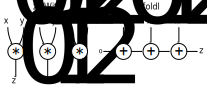
\includegraphics[width=3in]{HOFs}
    \caption{Structure of \emph{zipWith} and \emph{foldl}}
    \label{fig:zipwthandfoldlstruct}
  \end{figure}

  Functional specifications of computations can be represented by CSDF graphs using a straightforward translation.
  As an example, consider the functional specification of a simple dot product of two vectors, written in the functional programming language Haskell:

\begin{verbatim}
dotp xs ys = fold (+) 0 (zipWith (*) xs ys)  
\end{verbatim}


  The CSDF graph representation of this specification is depicted in Figure~\ref{fig:csdf-dotproduct}.
  Each node in the graph represents a function, where function is to be interpreted in the widest sense: we regard values simply as functions that take no argument.
  The node corresponding to the addition has a self-loop, which indicates that it is involved in a \emph{stateful} computation - the fold.
  Note that neither of the two higher-order functions that appear in the specification (fold and zipWith) are represented by nodes in the CSDF graph.
  Higher-order functions do not map to individual nodes, but rather to \emph{subgraphs}.
  In general, the CSDF graphs derived from functional specifications are \emph{hierarchical}.
  That is, one may collapse a subgraph into a single node, which makes the higher-order functions explicit.

  \begin{figure}[h!]
    \centering
    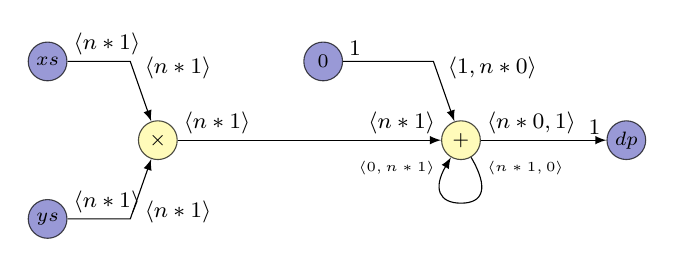
\begin{tikzpicture}[xscale=0.7]

\tikzstyle{sdfgnode} = [circle,draw=black,draw opacity=0.7,fill=yellow!30,fill opacity=0.9,inner sep=0,minimum width=14pt,font=\scriptsize,text=black,text opacity=1]%
\tikzstyle{sdfgdata} = [sdfgnode, inner sep=1pt,fill=blue!60!black,fill opacity=0.4]%
\tikzstyle{sdfgmem} = [sdfgnode, rectangle, rounded corners=4pt, inner sep=2pt,fill=blue!60!black,fill opacity=0.1]%
\tikzstyle{sdfgarc} = [->,minimum width=1pt,>=latex,sloped]%
\tikzstyle{token} = [circle,inner sep=0,draw=black,fill=black,minimum size=5pt]%
\tikzstyle{rate} = [inner sep=2pt,font=\footnotesize]%
\tikzstyle{bb} = [rectangle, draw=black!20, dashed]%

\node[sdfgdata] (xs) at (-1.5, 1) {$xs$};
\node[sdfgdata] (ys) at (-1.5, -1) {$ys$};
\node[sdfgnode] (mul) at (0.5, 0) {$\times$};

\node[sdfgdata] (a) at (3.5, 1) {0};
\node[sdfgnode] (f) at (6, 0) {$+$};
\node[sdfgdata] (w) at (9, 0) {$dp$};
%\node[sdfgdata] (x) at (2.5, 0) {$ps$};

\draw[sdfgarc] (xs) --
    node[pos=0.0,sloped,rate,anchor=south west] {$\langle n * 1 \rangle$}
    +(1.5, 0) --
    node[pos=0.4,sloped=false,rate,anchor=south west] {$\langle n * 1 \rangle$}
    (mul);

\draw[sdfgarc] (ys) --
    node[pos=0.0,sloped,rate,anchor=south west] {$\langle n * 1 \rangle$}
    +(1.5, 0) --
    node[pos=0.4,sloped=false,rate,anchor=north west] {$\langle n * 1 \rangle$}
    (mul);

\draw[sdfgarc] (mul) --
    node[pos=0.0,sloped,rate,anchor=south west] {$\langle n * 1 \rangle$}
    node[pos=1.0,sloped=false,rate,anchor=south east] {$\langle n * 1 \rangle$}
    (f);

\draw[sdfgarc] (a) --
    node[pos=0.0,sloped,rate,anchor=south west] {$1$}
    +(2, 0) --
    node[pos=0.4,sloped=false,rate,anchor=south west] {$\langle 1, n * 0 \rangle$}
    (f);

%\draw[sdfgarc] (x) --
%    node[pos=0.0,sloped,rate,anchor=south west] {$\langle n * 1 \rangle$}
%    node[pos=0.9,sloped=false,rate,anchor=south east] {$\langle 0, n * 1 \rangle$}
%    (f);

\draw[sdfgarc] (f) --
    node[pos=0.0,rate,anchor=south west] {$\langle n * 0, 1 \rangle$}
    node[pos=1.0,rate,anchor=south east] {$1$}
    (w);

\begin{scope}[scale=0.8]
\draw[sdfgarc] (f)
    .. controls ($(f) + (-50:1)$) and ($(f) + (0.5,-1)$) .. ($(f) + (0, -1)$)
    node[pos=0.3, sloped=false, rate, anchor=south west, font=\tiny] {$ \langle n * 1, 0 \rangle $}
    .. controls ($(f) + (-0.5,-1)$) and ($(f) + (-130:1)$) ..
    node[pos=0.7, sloped=false, rate, anchor=south east, font=\tiny] {$ \langle 0, n * 1 \rangle $}
    (f);
\end{scope}

\end{tikzpicture}

    \caption{Cyclo-static dataflow graph representation of dot-product.}
    \label{fig:csdf-dotproduct}
  \end{figure}

  Each node in the CSDF graph represents a function that is computed at a particular \emph{place} - a location in space, such as a processing element, or an input port.
  Performing the computation on actual values corresponds to \emph{executing} the CSDF graph.
  During such an execution, each node may be invoked several times, at different time instants.

  By applying an \emph{unfolding} transformation to the graph, a node is replaced by several copies, each representing a subset of the invocations of that node.
  This increases the space allocated to that function, and decreases the number of node invocations per place.
  It furthermore explicitly exposes parallelism, which may be beneficial to performance.
  
  In order to determine performance metrics of an application, the simulation must be accurate.
  In SDFkit, the simulation can be used to verify functional correctness as well as performance.
  Due to a specific mapping of the application graph to hardware, a cycle accurate simulation can be performed.
  Additionally, the tokens on the edges can be changed any time allowing the user to identify bottlenecks in the graph and to tweak performance.
  
  During hardware generation, each node is implemented as a combinational circuit containing the functionality of the node and logic for producing and consuming data.
  The edges, on the other hand, are implemented as FIFOs.
  The code is generated using \clash, a functional hardware description language~\cite{Baaij10}.
  Additional to the python code in a node for simulation, \clash\ code is added for the implementation on hardware.


\section{Results}
\label{sec:results}

  Currently, SDFkit can import graphs expressed in a JSON file containing a list of nodes and edges.
  Additionally, each node contains a python lambda expression for the functional behavior of the node during simulation.
  After opening, both the functionality of the nodes and data on the edges can be altered using the GUI.

  Figure \ref{fig:screenshot} shows a screenshot of SDFkit.
  The central widget shows a visualization of a CSDF graph which can be simulated in a step-wise fashion using the control panel on the left.
  For debugging purposes, the data in tokens is visualized in the lower widget.

  \begin{figure}[h!]
    \centering
    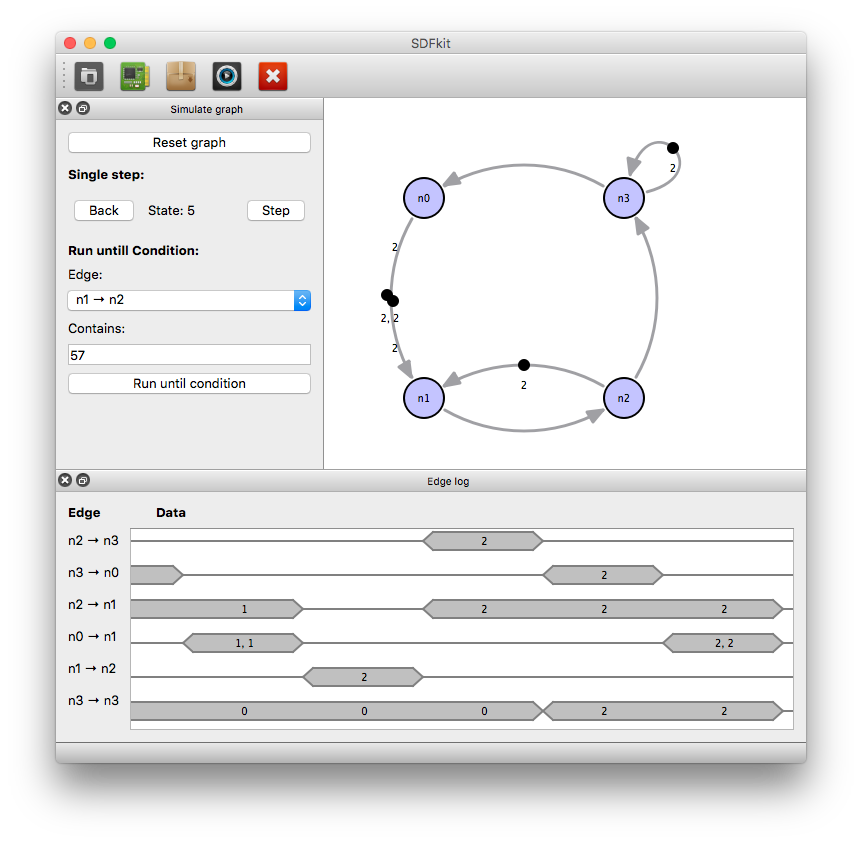
\includegraphics[width=3in]{screenshot.png}
    \caption{Screenshot of SDFkit}
    \label{fig:screenshot}
  \end{figure}

  Currently, the hardware generation backend only supports \emph{homogeneous} SDF (HSDF) graphs, which is the simplest type of SDF graph.
  To support CSDF graphs, the edges have to support storing a variable amount of tokens each clock cycle which results in more complicated hardware.

\section{Conclusions and future work}
\label{sec:conclusions}

  In this paper we presented a methodology and an application for designing hardware using a structured approach.
  In contrast to translating imperative programming constructs like for-loops to hardware, we use constructs to express the structure in a computation.
  Using these computational structures, the generation of highly parallel hardware is tremendously simplified.
  Applications are modeled using CSDF graphs which are a cycle-accurate model for the generated hardware.
  This methodology is currently being implemented in SDFkit, an interactive simulation and hardware generation environment supporting visualization and simulation of CSDF graphs.
  Additionally, \clash\ code can be generated for HSDF graphs.

  The next step in development is to extend the hardware code generation with support for CSDF graphs.
  Additionally, the transformations to make a tradeoff between space and time are now performed outside SDFkit.
  Integration of these transformations into SDFkit is therefore an other important step forward.
  Finally, interesting opportunities lie in extending the code generation with a wider range of supported platform like C code and OpenCL.
  
% Can use something like this to put references on a page
% by themselves when using endfloat and the captionsoff option.
\ifCLASSOPTIONcaptionsoff
  \newpage
\fi



% trigger a \newpage just before the given reference
% number - used to balance the columns on the last page
% adjust value as needed - may need to be readjusted if
% the document is modified later
%\IEEEtriggeratref{8}
% The "triggered" command can be changed if desired:
%\IEEEtriggercmd{\enlargethispage{-5in}}

% references section

% can use a bibliography generated by BibTeX as a .bbl file
% BibTeX documentation can be easily obtained at:
% http://www.ctan.org/tex-archive/biblio/bibtex/contrib/doc/
% The IEEEtran BibTeX style support page is at:
% http://www.michaelshell.org/tex/ieeetran/bibtex/
%\bibliographystyle{IEEEtran}
% argument is your BibTeX string definitions and bibliography database(s)
%\bibliography{IEEEabrv,../bib/paper}
%
% <OR> manually copy in the resultant .bbl file
% set second argument of \begin to the number of references
% (used to reserve space for the reference number labels box)
% \begin{thebibliography}{1}

% \bibitem{IEEEhowto:kopka}
% H.~Kopka and P.~W. Daly, \emph{A Guide to \LaTeX}, 3rd~ed.\hskip 1em plus
%   0.5em minus 0.4em\relax Harlow, England: Addison-Wesley, 1999.

%   \bibliographystyle{unsrt}
% {\small\bibliography{biblio}}


% \end{thebibliography}

% bibliography{IEEEabrv,biblio}

\bibliographystyle{unsrt}
\bibliography{biblio}

% You can push biographies down or up by placing
% a \vfill before or after them. The appropriate
% use of \vfill depends on what kind of text is
% on the last page and whether or not the columns
% are being equalized.

%\vfill

% Can be used to pull up biographies so that the bottom of the last one
% is flush with the other column.
%\enlargethispage{-5in}

\end{document}


